%% Author: Daniel Kaplan
%% Subject: Shapes of models





The drawings show some data involving three variables:
\begin{itemize}
  \item D --- a quantitative variable
  \item A --- a quantitative variable
  \item G --- a categorical variable with two levels: S \& K
\end{itemize}
On each of the plots, sketch a graph of the fitted model function of the indicated structure.


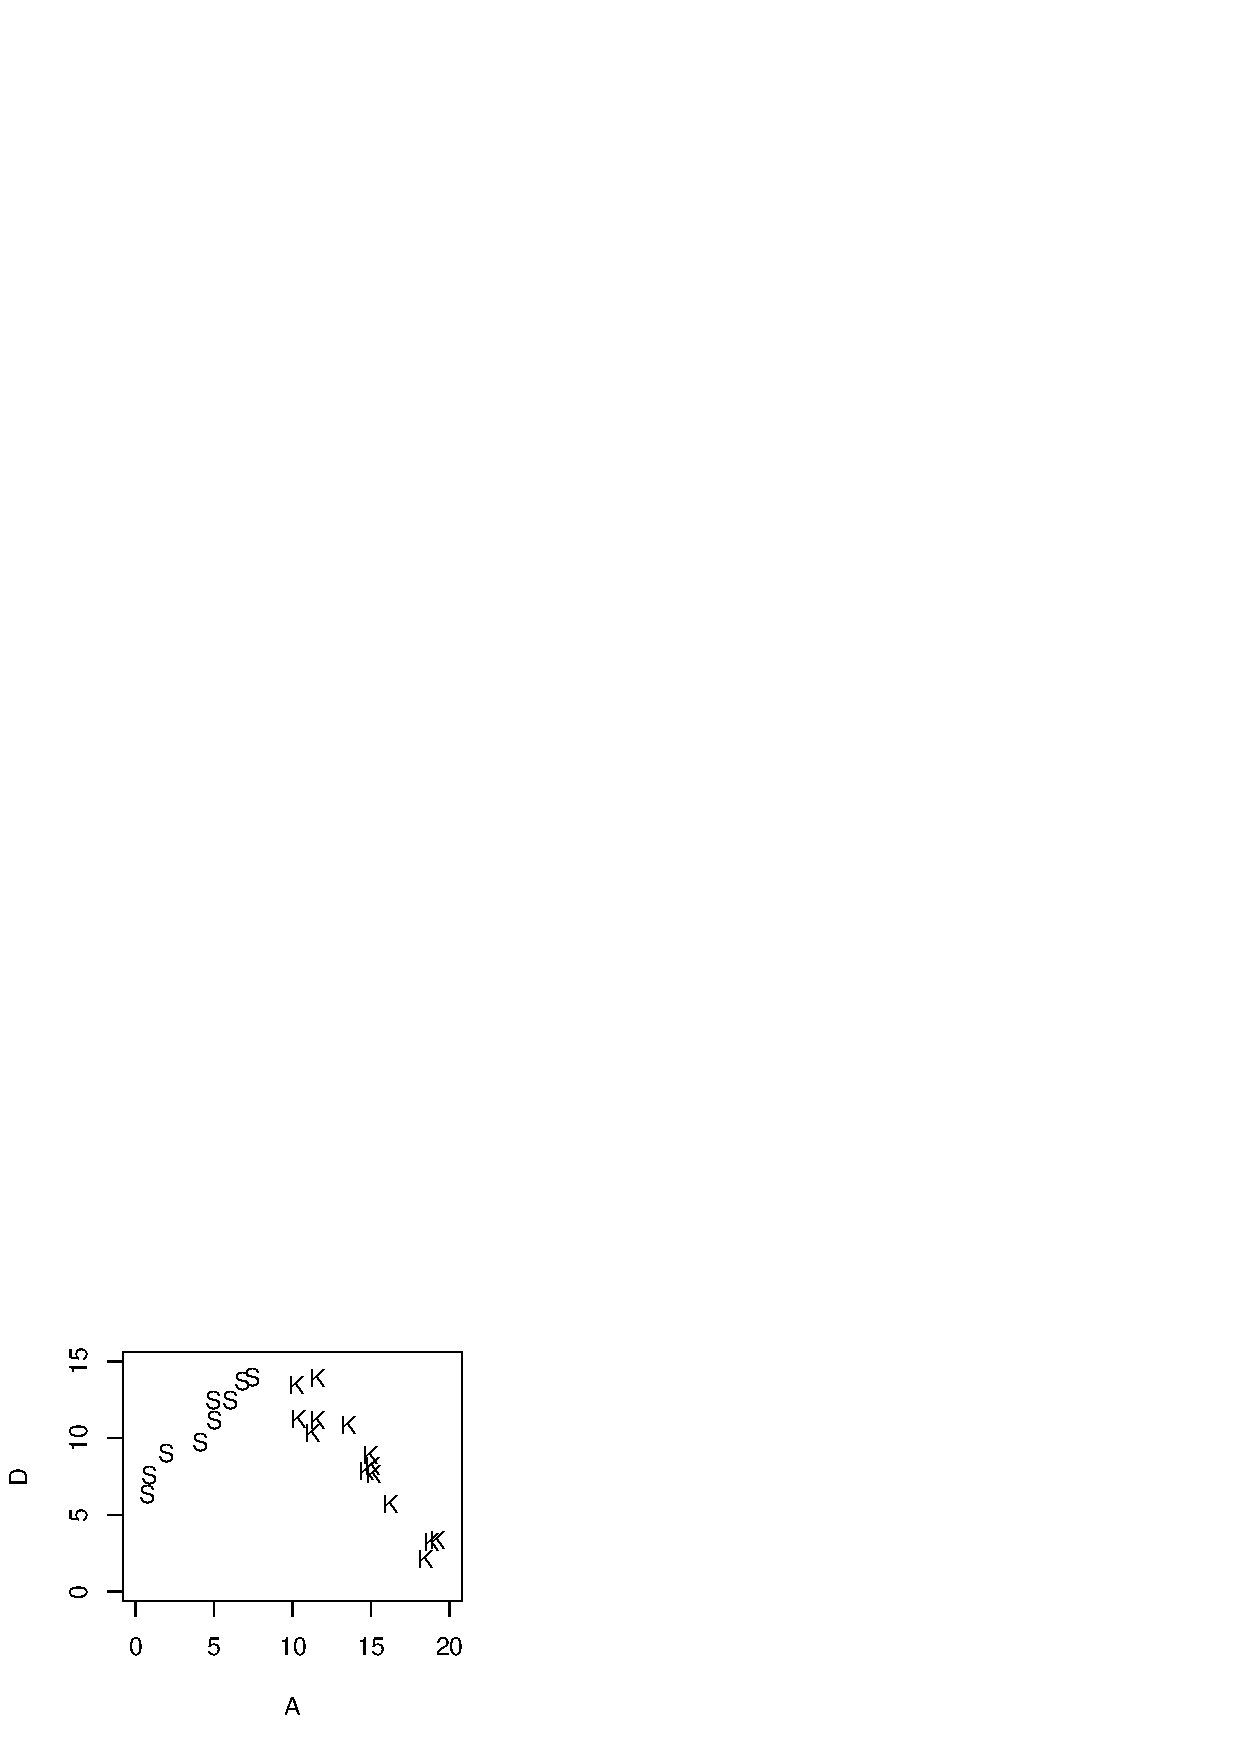
\includegraphics{Figures/fig-fig-4-3-main}


Draw these models:
\begin{itemize}
  \item \verb-D ~ A+G-
    
\begin{AnswerText}
\includegraphics{Figures/fig-fig-4-3-q1}
\end{AnswerText}

 \item \verb=D ~ A*G=

\begin{AnswerText}
\includegraphics{Figures/fig-fig-4-3-q2}
\end{AnswerText}

\item \verb=D ~ A-1=
   
\begin{AnswerText}
\includegraphics{Figures/fig-fig-4-3-q3}
\end{AnswerText}


 \item \verb-D ~ 1-
   

\begin{AnswerText}
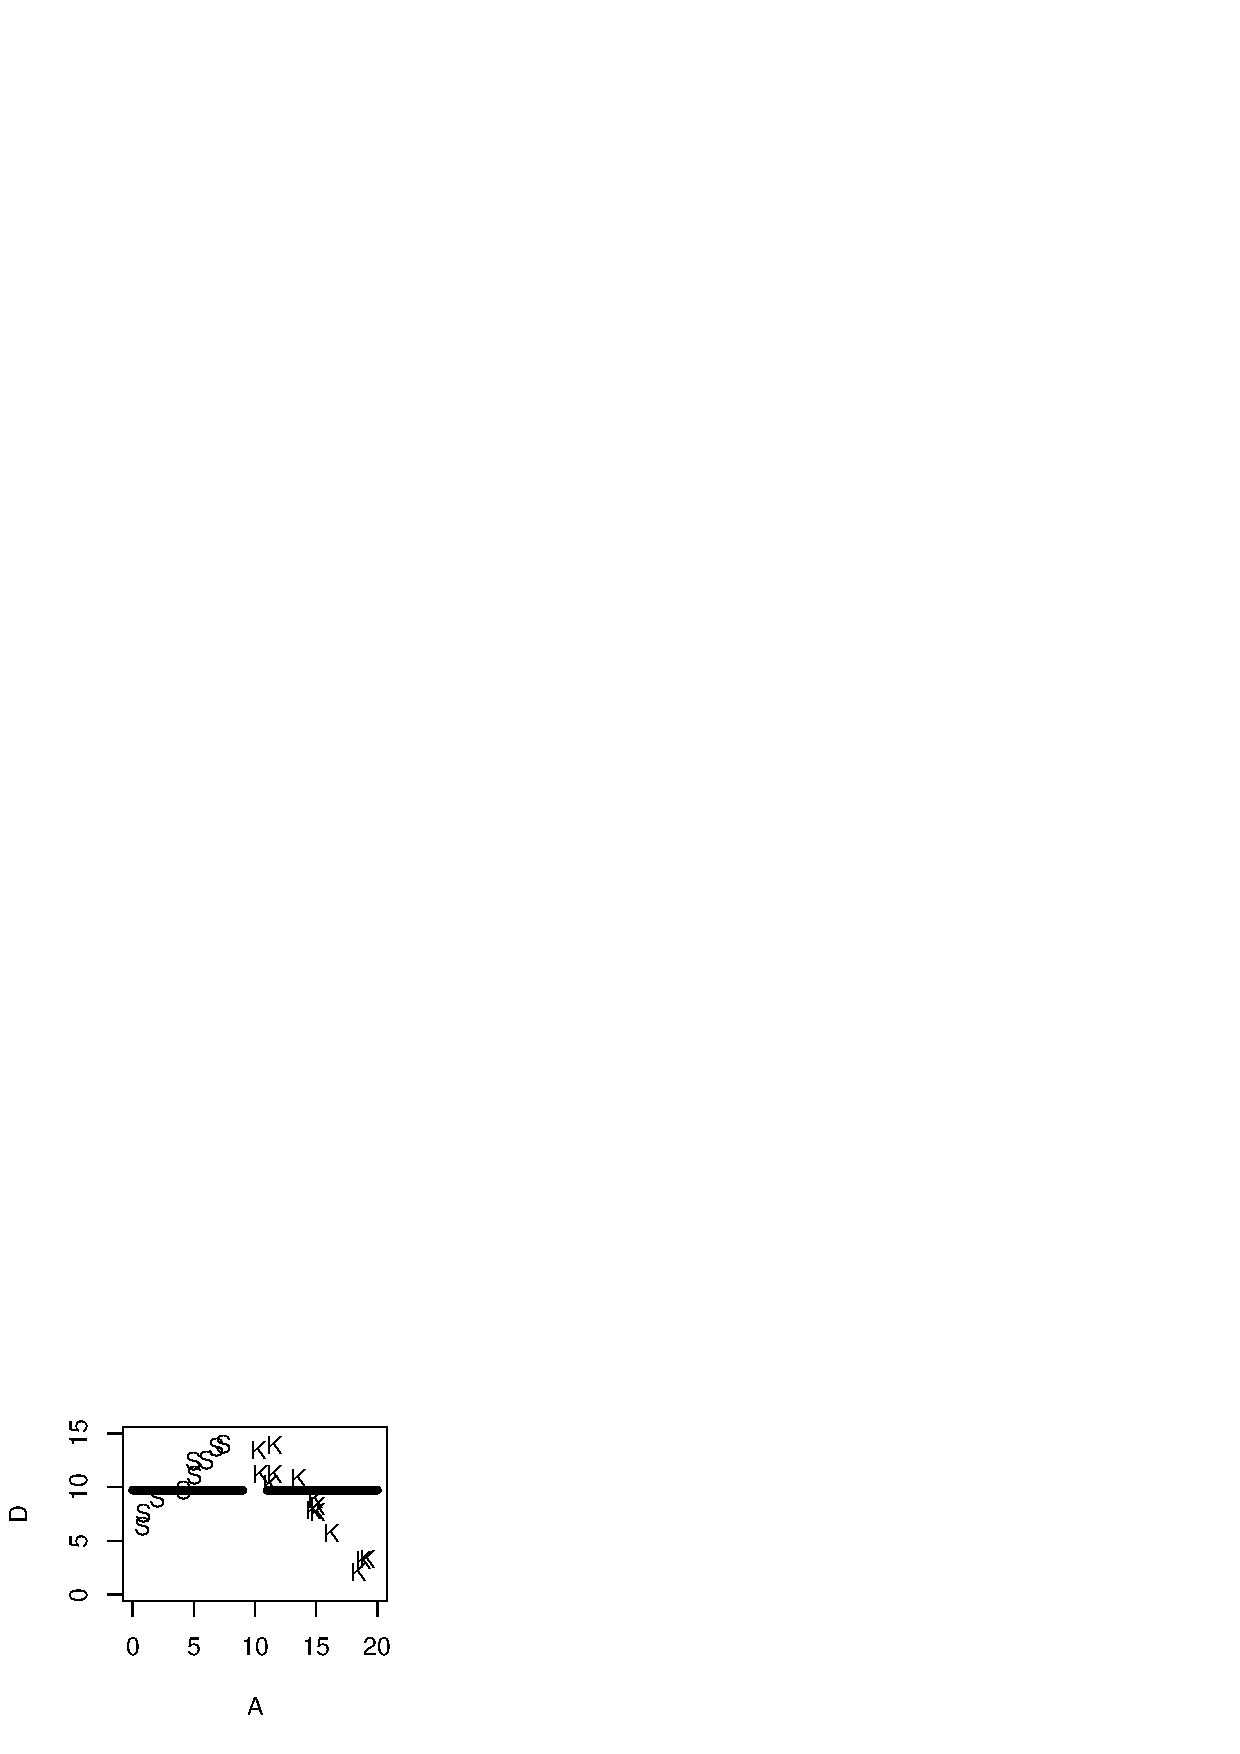
\includegraphics{Figures/fig-fig-4-3-q4}
\end{AnswerText}
   
   
   
  \item \verb-D ~ A-
   
\begin{AnswerText}
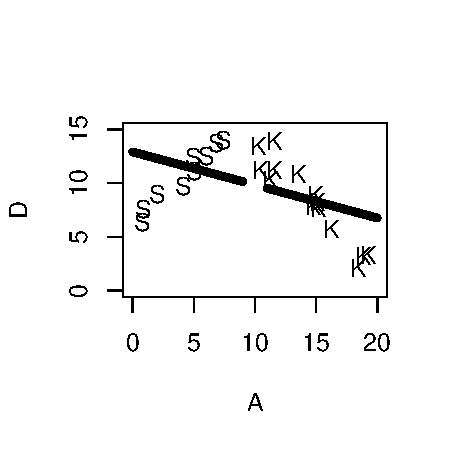
\includegraphics{Figures/fig-fig-4-3-q5}
\end{AnswerText}


  
  
\item D \verb=~= poly(A,2)

\begin{AnswerText}
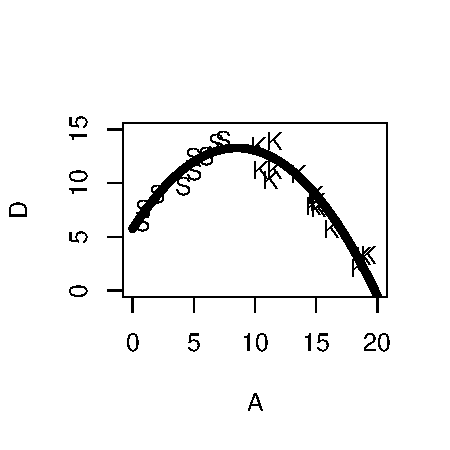
\includegraphics{Figures/fig-fig-4-3-q6}
\end{AnswerText}


  
  \end{itemize}
Only a qualitative sketch is needed.  It will be good enough to draw
out the graph on a piece of paper, roughly approximating the patterns
of S and K seen in the graph.  Then draw the model values right on
your paper.  (You can't hand this in with AcroScore.)
  
  
\bigskip
  
  
Example: \verb+D ~ G+

\includegraphics{Figures/fig-fig-4-3-ex1}

